\section{Introducción y Objetivo}

La \textbf{distribución de energía eléctrica} es un componente vital, siendo el enlace final entre la generación y el consumidor. La topología de la red es determinante en la \textbf{calidad, continuidad del servicio y costo}. Históricamente, han prevalecido las configuraciones \textbf{radial} y \textbf{en anillo} (o bucle). La elección depende de la densidad de carga, la importancia crítica de los usuarios y las restricciones presupuestarias.

El objetivo principal es \textbf{definir, comparar y analizar las características operativas y de diseño}, así como las ventajas y desventajas inherentes, de los sistemas de distribución eléctrica con configuración radial y en anillo.

\section{Desarrollo y Análisis Comparativo de Redes}

\subsection{Definición de Redes}

\subsubsection{Red de Distribución Radial}
Caracterizada por presentar un \textbf{solo camino} para el flujo de potencia. Si el camino se interrumpe, resulta en la \textbf{pérdida total del servicio} para los clientes ``río abajo''.

\subsubsection{Red de Distribución en Anillo (Loop)}
Diseñada para ofrecer \textbf{más de un camino} para el flujo de potencia. A menudo se opera como un \textbf{bucle abierto} (operacionalmente radial), pero mantiene la capacidad de reconfiguración.

\subsection{Comparación de Características Clave}

\begin{table*}[h!]
  \centering
  \caption{Comparación de Características: Radial vs. En Anillo}
  \label{tab:comparacion_redes_resumen}
  \begin{tabular}{p{0.3\textwidth} p{0.3\textwidth} p{0.3\textwidth}}
    \toprule
    \textbf{Característica} & \textbf{Red Radial (Radial)} & \textbf{Red en Anillo (Loop)} \\
    \midrule
    \textbf{Ventajas} &
    \begin{itemize}
      \item \textbf{Costo más bajo} y simple.
      \item Operación y protección sencillas.
      \item Flujos de potencia predecibles.
    \end{itemize} &
    \begin{itemize}
      \item \textbf{Mayor fiabilidad} y continuidad de servicio.
      \item Las fallas interrumpen un segmento mínimo (redirección).
      \item Alimentación posible desde dos direcciones.
    \end{itemize} \\
    \midrule
    \textbf{Desventajas} &
    \begin{itemize}
      \item \textbf{Menos fiable}.
      \item Una falla interrumpe el servicio a todos los clientes aguas abajo.
    \end{itemize} &
    \begin{itemize}
      \item \textbf{Más costoso} (mayor inversión inicial).
      \item Requiere conductor y equipo de mayor capacidad (doble capacidad).
      \item Análisis y operación ligeramente más complejos.
    \end{itemize} \\
    \midrule
    \textbf{Usos Comunes} &
    \begin{itemize}
      \item \textbf{Diseño más utilizado} (predominante).
      \item Zonas habitacionales/comerciales no críticas.
      \item Cargas ligeras y áreas de densidad media.
    \end{itemize} &
    \begin{itemize}
      \item \textbf{Cargas Críticas} (e.g., hospitales).
      \item Grandes Cargas Urbanas o distribución subterránea.
      \item Donde la continuidad es primordial.
    \end{itemize} \\
    \bottomrule
  \end{tabular}
\end{table*}

\subsection{Diferencias Operacionales y Estructurales}

\begin{enumerate}
\item \textbf{Topología y Caminos de Flujo:} \textbf{Radial} tiene una \textbf{única trayectoria}; \textbf{Anillo} tiene \textbf{al menos dos} trayectorias.
\item \textbf{Costo y Capacidad:} \textbf{Radial} es el de menor costo y más simple. \textbf{Anillo} es más costoso y requiere conductores de mayor capacidad para soportar la carga desde ambos extremos.
\item \textbf{Manejo de Fallas y Fiabilidad:} En \textbf{Radial}, una falla interrumpe el servicio aguas abajo. En \textbf{Anillo}, la fiabilidad es mayor: la sección con falla se aísla rápidamente, manteniendo el servicio por la dirección alternativa.
\item \textbf{Complejidad de Análisis:} Los flujos \textbf{Radiales} son predecibles. La red \textbf{Anillo} (operada cerrada) requiere técnicas de red más complejas para análisis.
\end{enumerate}

\section{Ejemplos en Planos y Diagramas Unifilares}

Para cumplir con la visualización de las topologías, se presentan los diagramas unifilares simplificados de las redes Radial y En Anillo.

\subsection{Red de Distribución Radial}
Esta topología se caracteriza por un \textbf{flujo de potencia unidireccional} desde la subestación hasta el último punto de carga, sin rutas alternativas.

\begin{figure}[ht!]
    \centering
    % DEBES REEMPLAZAR 'radial_network_diagram.png' con el nombre de tu archivo de imagen
    % Asegúrate de tener la imagen en tu carpeta o usa el comando \includegraphics{} apropiado para el link si es posible.
    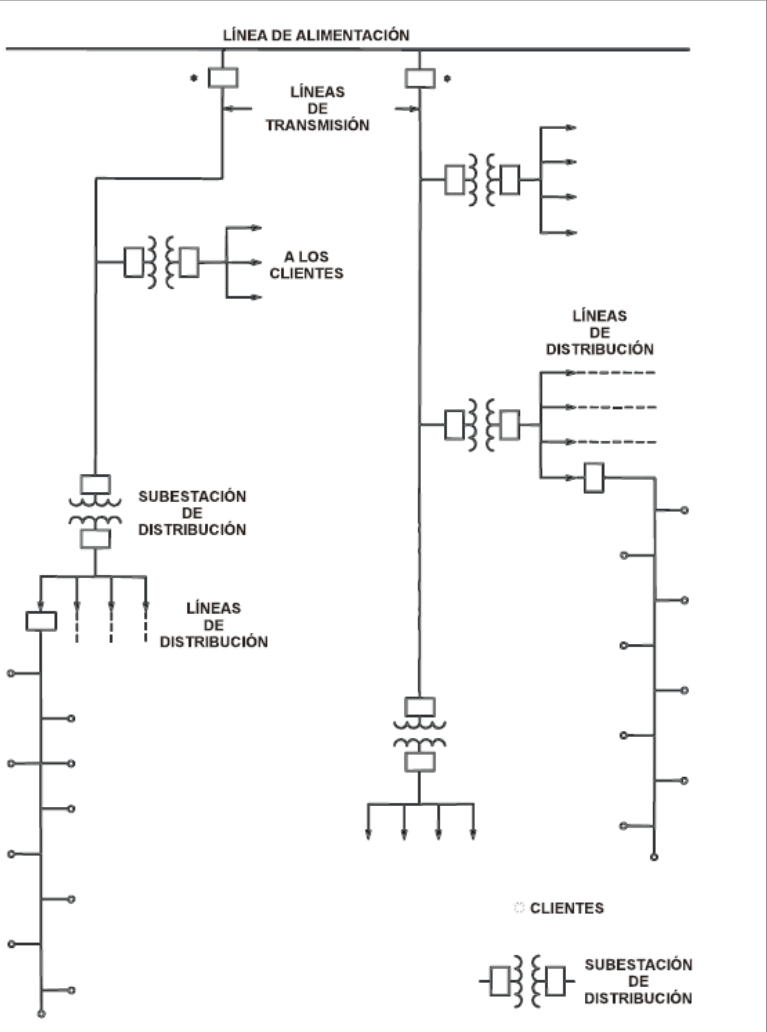
\includegraphics[width=0.45\textwidth]{fig_/radial_network_diagram.png} 
    \caption{Diagrama Unifilar de una Red de Distribución Radial.}
    \label{fig:radial_unifilar}
\end{figure}

\subsubsection*{Análisis y Referencia}
Una falla en cualquier punto intermedio interrumpe el servicio a todos los usuarios aguas abajo. Un diagrama representativo se puede consultar en la colección: \url{https://www.researchgate.net/figure/Figura-1-Diagrama-de-una-red-de-distribucion-radial_fig1_359246177}

\vspace{0.5cm}
\hrule
\vspace{0.5cm}

\subsection{Red de Distribución en Anillo (Operación Abierta)}
Aunque la red está conectada físicamente en un bucle, se opera normalmente \textbf{abierta} en un punto (Seccionador N.A. - Normalmente Abierto). Esto permite la \textbf{reconfiguración} para aislar fallas sin perder el servicio en las cargas críticas.

\begin{figure}[ht!]
    \centering
    % DEBES REEMPLAZAR 'ring_network_diagram.png' con el nombre de tu archivo de imagen
    % Asegúrate de tener la imagen en tu carpeta o usa el comando \includegraphics{} apropiado para el link si es posible.
    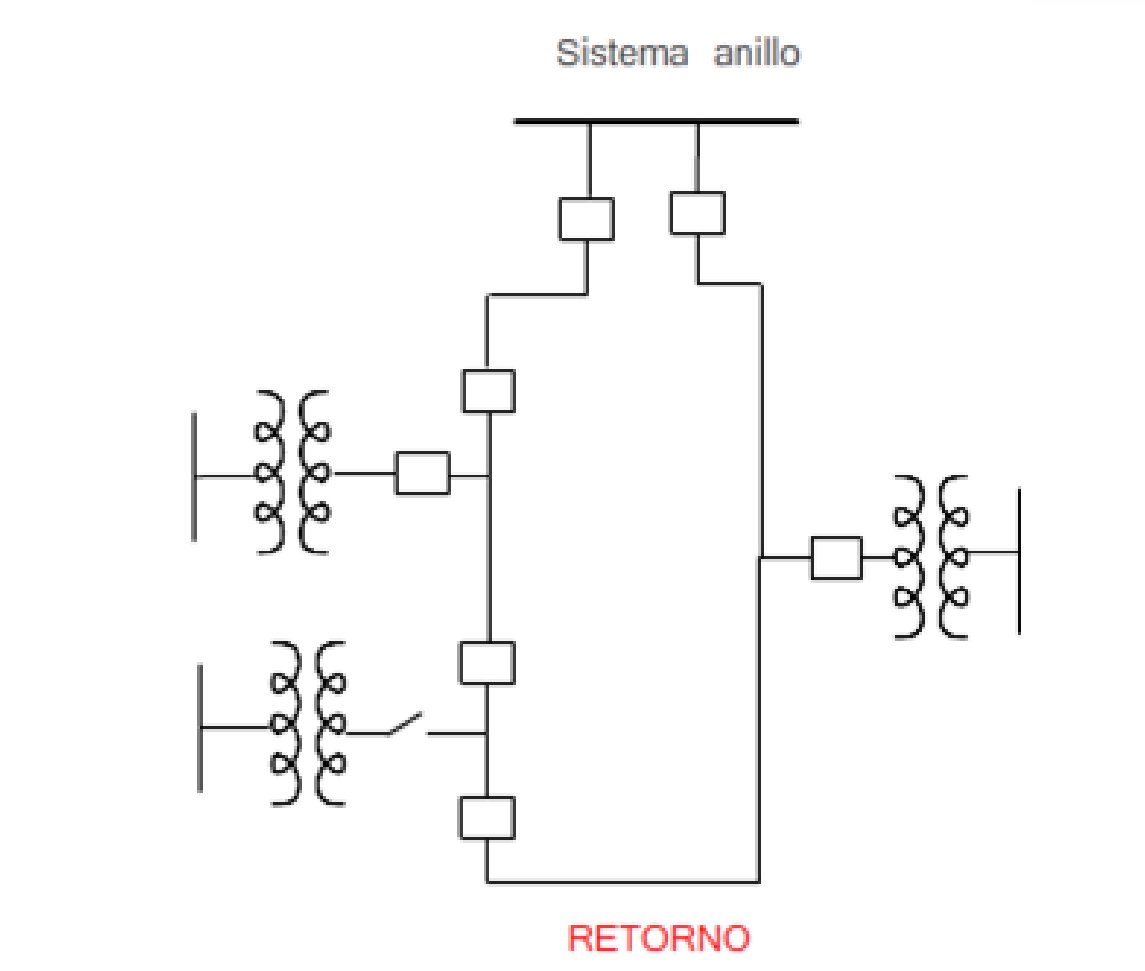
\includegraphics[width=0.45\textwidth]{fig_/ring_network_diagram.png} 
    \caption{Diagrama Unifilar de una Red en Anillo (Operación Normalmente Abierta).}
    \label{fig:anillo_unifilar}
\end{figure}

\subsubsection*{Análisis y Referencia}
En caso de falla, el punto N.A. se cierra y el punto de falla se aísla, manteniendo la alimentación por el camino alternativo, lo que garantiza una mayor fiabilidad. Un diagrama representativo se puede consultar en la colección: \url{http://www.ptolomeo.unam.mx:8080/xmlui/bitstream/handle/132.248.52.100/784/A4%20SISTEMAS%20DE%20DISTRIBUCION.pdf?sequence=4}


\section{Conclusiones}

La decisión es un balance directo entre el \textbf{costo inicial} y la \textbf{continuidad del servicio} deseada.

\begin{itemize}
    \item La red \textbf{Radial} es la opción predominante por su \textbf{simplicidad operativa y bajo costo}, sacrificando fiabilidad (falla = interrupción inevitable).
    \item La red \textbf{En Anillo} es la solución ideal para \textbf{cargas críticas y áreas de alta densidad}, ofreciendo alta \textbf{resiliencia} a pesar de la mayor inversión y complejidad de análisis.
\end{itemize}

En la práctica, los sistemas radiales comúnmente incorporan lazos de interconexión (normally open ties) para aumentar su flexibilidad, combinando la economía del diseño radial con un nivel básico de redundancia.